\chapter{Charts \& Tables}
\section{Skill Roll Outcome Graph}
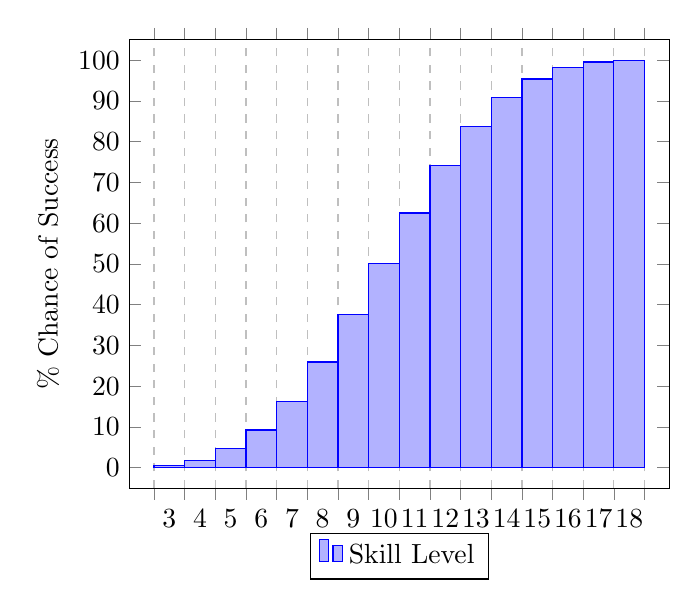
\begin{tikzpicture}
\begin{axis}[
	x tick label style={/pgf/number format/1000 sep=},
	ylabel=\% Chance of Success,
	enlargelimits=0.05,
	ytick = {0, 10, 20, 30, 40, 50, 60, 70, 80, 90, 100},
	legend style = {
	    at={(0.5,-0.1)},
	    grid style = dashed,
	    anchor=north,legend columns=-1
	},
	ybar interval = 1,
]
\addplot 
	coordinates {
	    (3, 0.46) 
	    (4, 1.85)
		(5, 4.63) 
		(6, 9.26) 
		(7, 16.20) 
		(8, 25.93) 
		(9, 37.50) 
		(10, 50.00) 
		(11, 62.50) 
		(12, 74.07)
		(13, 83.80)
		(14, 90.74)
		(15, 95.37)
		(16, 98.15)
		(17, 99.54)
		(18, 100.00)
		(19, 0)
	};
\legend{Skill Level}
\end{axis}
\end{tikzpicture}\\
The graph above shows the probability of succeeding a skill roll. If your character has an effective skill of 10, they have a 50\% chance of succeeding that roll. If they have a skill of 12, the chance of success goes up to 74\%.